\documentclass{article}

% ---- NeurIPS 2026 style ----
% Tracks (uncomment exactly one). Default = main track, double-blind submission.
\usepackage{neurips_2026}
% \usepackage[main]{neurips_2026}
% \usepackage[position]{neurips_2026}
% \usepackage[eandd]{neurips_2026}
% \usepackage[creativeai]{neurips_2026}
% \usepackage[sglblindworkshop]{neurips_2026}
% \usepackage[dblblindworkshop]{neurips_2026}
%
% After acceptance, append `final` to the chosen track to compile camera-ready:
%   \usepackage[main, final]{neurips_2026}
%
% For arXiv / non-anonymous preprint:
%   \usepackage[preprint]{neurips_2026}

% ---- Additional packages (natbib is loaded by neurips_2026.sty) ----
\usepackage[utf8]{inputenc}
\usepackage[T1]{fontenc}
\usepackage{hyperref}
\usepackage{url}
\usepackage{booktabs}
\usepackage{amsmath,amssymb,amsfonts}
\usepackage{nicefrac}
\usepackage{microtype}
\usepackage{xcolor}
\usepackage{graphicx}
\usepackage{multirow}
\usepackage{makecell}
\usepackage{subcaption}
\usepackage{algorithm}
\usepackage{algorithmic}

\hypersetup{
  colorlinks=true,
  linkcolor=blue!70!black,
  citecolor=green!50!black,
  urlcolor=blue!70!black
}

% ---- Custom commands ----
\newcommand{\method}{ESR}
\newcommand{\Method}{ESR}
\newcommand{\methodfull}{Early Stopping Rollout}
\newcommand{\KL}{\mathrm{KL}}
\newcommand{\bboxed}{\texttt{\textbackslash boxed\{\}}}
\newcommand{\tbd}[1]{\textcolor{red}{[TBD: #1]}}
\newcommand{\beatsteacher}{\textcolor{red!85!black}{$\bigstar$}}

\title{Less is More: Early Stopping Rollout for \\ On-Policy Distillation}

% NeurIPS 2026 author block.
% At submission time the default (anonymous) option hides the author block
% automatically; fill in real names/affiliations only for `final` or
% `preprint` compilations.
\author{%
  Anonymous Authors\\
  % Affiliation \\
  % Address \\
  % \texttt{email} \\
  % examples of more authors:
  % \And
  % Coauthor \\
  % Affiliation \\
  % Address \\
  % \texttt{email} \\
}

\begin{document}

\maketitle

% ============================================================================
% ABSTRACT
% ============================================================================
\begin{abstract}
% On-policy distillation scores every token of the student's rollout with the teacher. We identify a subtlety that changes the picture: the teacher's score at position $t$ is conditioned on the student's own previously generated tokens, so early in a rollout the teacher judges \emph{how to approach the problem}, whereas later it can only judge \emph{how to continue what the student has already written}. Given a sufficiently long student rollout, the teacher's accuracy collapses toward the student baseline, indicating that late-position supervision is far weaker than early-position supervision. We therefore propose \emph{\methodfull{}} (\method{}): restrict both the rollout and the reverse-KL loss to the first $N$ response tokens. Across tasks, model families, LoRA and full fine-tuning, and a range of teacher scales, \method{} matches or exceeds full-sequence distillation nearly everywhere, sometimes surpasses the teacher, trains far faster with far less memory, and avoids the collapse modes of full-sequence training. The obvious explanation---\method{} as a proxy for high-KL or high-entropy tokens---fails: every scalar-saliency selector we tried underperforms \method{}, and most underperform plain full-sequence. Position is an independent, load-bearing axis---it is where the planning tokens live, and a short reverse-KL loss there is enough to improve the entire response.
On-policy distillation has recently emerged as a promising alternative to standard sequence-level imitation, training a student by scoring its own rollouts with a teacher model. However, one important limitation is observed in this paradigm: at each position, the teacher scores the student's next token conditioned on the student's own previous outputs. Early tokens are therefore judged mainly in the context of the original problem and reflect how the student approaches the problem, whereas later tokens are constrained by increasingly student-specific context and provide much weaker supervision. Based on this intuition, we propose \methodfull{} (\method{}), a simple yet effective distillation strategy that restricts both rollout generation and reverse-KL to the first $N$ response tokens. This position-focused objective emphasizes the tokens that encode planning and reasoning, rather than spending supervision budget on late tokens whose informational value rapidly degrades. Empirical experiments have proved that \method{} shows both surpassing performance with high efficiency under various models and training methods. It is also proved that the teacher collapses in sufficiently long rollouts suggesting that late-position supervision contributes little useful learning signal. We further investigate the mechanism behind this effect and show that position is a distinct and crucial dimension of supervision, not merely a proxy for token uncertainty or difficulty.  It establishes position-aware supervision as an important direction for understanding and advancing OPD in future studies.
\end{abstract}

% ============================================================================
% 1. INTRODUCTION
% ============================================================================
\section{Introduction}
\label{sec:intro}

On-policy distillation (OPD) has emerged as a dominant paradigm for model distillation in industrial practice. The student generates its own rollouts $\tau$, which are then scored by the teacher: at each token, the teacher's probability $\pi_{teacher}(\tau_{student} \mid x_{prompt})$ serves as the soft target for the student~\citep{agarwal2024onpolicy, gu2024minillm}.  Viewed through an RL lens, this is equivalent to using the teacher as a dense, token-level reward model that judges the student's own behavior on a given prompt. The final objective is then a simple \emph{uniform average} of the per-token reverse-KL across the trajectory.
  
This uniform averaging implicitly assumes that the teacher's signal is equally reliable at every position in the trajectory. We argue that this assumption is unfounded, and that it breaks down precisely because of the autoregressive structure of LLMs. At the first token, the teacher's score is conditioned only on the prompt: $\pi_{teacher}(\tau_{student}^{t=1} \mid x_{prompt})$ - indeed what we expect the teacher to score on. At a later position $m$, however, it becomes conditioned also on the student's own previously generated tokens: $\pi_{teacher}(\tau_{student}^{t=m} \mid x_{prompt}, \tau_{student}^{t=1:m})$. This conditioning context is off-policy to the teacher model and may even be out-of-distribution (OOD), and grows more so with position.

To probe how severe this drift is, we run a preliminary experiment that measures how the teacher behaves when continuing from an early-stopped student rollout. As shown in Figure~\ref{fig:motivation}, the teacher's quality collapses toward the student's within roughly 300 tokens. If the teacher's late-position signal is unreliable, the natural question is whether early tokens alone are systematically more informative --- and whether training on them is sufficient.

Motivated by this, we propose \methodfull (\method): restrict the student rollout to its first $N$ tokens (e.g., 50 or 100) and compute the distillation loss only on this early window. The change is a single line in any on-policy distillation loop. Despite its simplicity, \method consistently outperforms full-rollout OPD across tasks (math, code, function calling), training regimes (LoRA, full fine-tuning), model scales (students 1.5B--7B, teachers 1.7B--14B), and model families (Qwen, Gemma), while reducing wall-clock cost by up to $24\times$ and peak training memory by up to $4\times$. We further observe that full-rollout OPD frequently destabilizes and collapses during training, whereas \method does not collapse in any of our settings. Perhaps most surprisingly, although the student is normally upper-bounded by the teacher's performance, \method-trained students often \emph{exceed} the teacher.

Such a small change yields such large gains probe us to investigate deeper. Firstly, we want to further validate whether the effectiveness of earlier tokens is intrinsically caused by better KL and entropy signals, because we also find that early tokens generally have larger KL and entropy. We test selectors that pick tokens by high KL, high entropy or combined regardless of position; all underperform \method, with most underperforming full-rollout. Therefore, although we don't exclude KL and entropy as auxillary factors, we confirm that the position is a an independent factor rather a saliency proxy. Furthermore, we identified an additional important mechanism  \emph{Convergence Cascade}: after training on the early window, KL divergence on the \emph{untrained} late tokens also drops by 30--40\%. Therefore, the KL divergence does not have to see late positions to repair them.

Lastly, we investigated into why \method sometimes even \emph{exceeds} the teacher --- a stronger phenomenon we observe on most of our main experiment Table~\ref{tab:main_results}. We trace this to the mode-seeking nature of reverse-KL: the student commits to a subset of supported teacher modes instead of chasing all of them. Our \method loss helps it steer toward a non-dominant but correct mode rather than the teacher's argmax. Empirically, we find \method-trained students commit harder to their own choices than full-rollout students yet agree \emph{less} with the teacher's argmax, and produce trajectories ${\sim}3\times$ shorter than full-rollout and ${\sim}2\times$ shorter than the base student (\S\ref{sec:mode_seek}). It learns the teacher's strategy but preserves its succinct style, leading to better compount behaviors. This finding showcases a potential path of superceding the teacher model in distillation that worth further investigations.

Our contributions are summarized below:
\begin{enumerate}
    \item \textbf{\methodfull (\method) outperforms full-rollout on-policy distillation.} A one-line change---restricting the rollout length to the first $N$ response tokens---beats full-sequence distillation across tasks, model families, scales, and training regimes, while being dramatically more efficient and far more stable to train. It can even exceed the teacher's own performance (Sections~\ref{sec:method}--\ref{sec:stability}).
    \item \textbf{A systematic investigation of why it works.} First, through a token-selection ablation, we show that the gain is not ``high KL'' or ``high entropy'' in disguise: position itself is a load-bearing axis. We also identify convergence cascading to be another important mechanism. Furthermore, we explain why \method often surpasses the teacher: by exploiting the mode-seeking behavior of reverse-KL training, \method pushes the student toward a better, non-dominant sub-mode (Section~\ref{sec:mechanisms_section}).
\end{enumerate}


% ============================================================================
% 2. MOTIVATION
% ============================================================================
\begin{figure}[t]
    \centering
    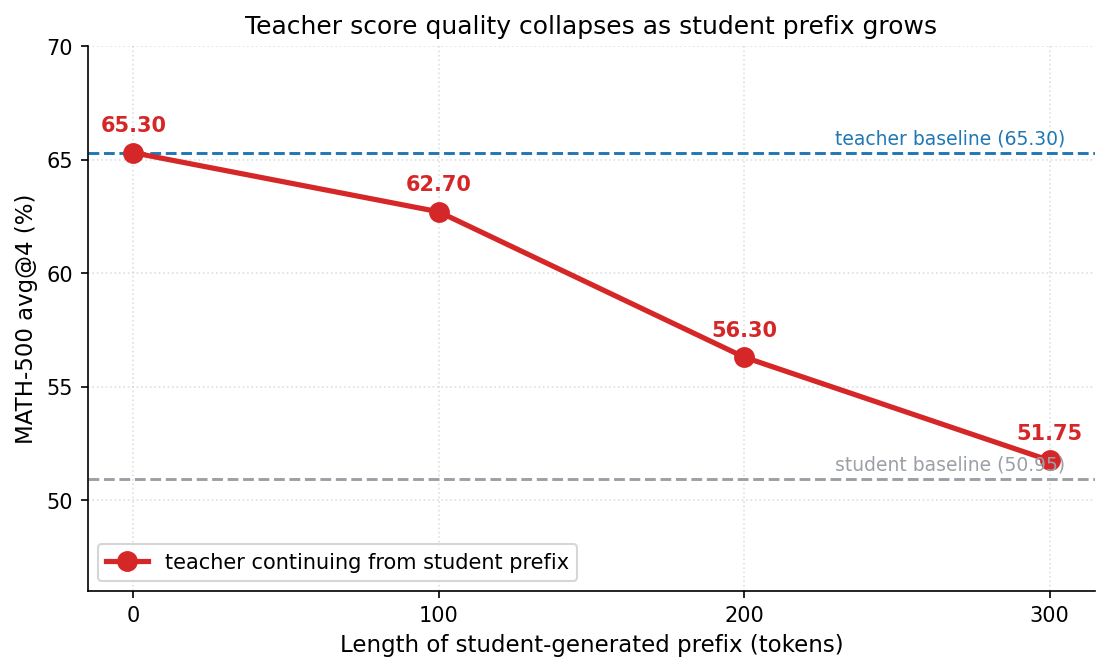
\includegraphics[width=0.7\textwidth]{figures/motivation_prefix_curve.png}
    \caption{\textbf{The teacher loses accuracy quckly as the student-generated rollout grows in a few hundred of tokens.} MATH-500, avg@4 ($n{=}4$, $t{=}0.7$). Teacher = Qwen3-1.7B; student = Qwen2.5-Math-1.5B. After $\sim$300 student tokens the teacher has effectively been dragged down to student-baseline performance.}
    \label{fig:motivation}
\end{figure}
  
\section{Why Late-Position Supervision Is Unreliable}
\label{sec:motivation}

In on-policy distillation, the teacher model scores the student's rollout at each position $t$ via $\pi_t(\cdot \mid x, y_{<t}^{\text{student}})$ and averages these scores uniformly across the rollout. The conditioning context $y_{<t}^{\text{student}}$, however, is whatever this particular student happened to write at this particular moment of training. As $t$ grows it drifts away from any distribution the teacher itself was trained on---off-policy to the teacher and, for long enough or atypical enough rollouts, plausibly out-of-distribution. We term this problem as ``Off-policy Teacher Drift''.  

To verify the intuition, we feed the teacher a $k$-token student-generated rollout on MATH-500 and letting it continue autoregressively, the teacher's avg@4 ($n{=}4$, $t{=}0.7$) falls from its 65.30\% unconditional baseline to 62.70\% at $k{=}100$ and 51.75\% at $k{=}300$---essentially student-baseline (Figure~\ref{fig:motivation}). Late-position teacher scores are not independent assessments of the prompt; it is a guess at how to continue a trajectory the student has already committed to. 
  
The problem compounds during training because the student's policy is moving. Early on, the student's rollout is far from the teacher; late-position targets are fitted under a strongly off-policy prefix. As training progresses and earlier tokens approach the teacher's distribution, the right late-position behavior changes too---continuations that were sensible above an off-policy prefix are no longer sensible above an on-policy one. But the late-position habits learned earlier do not cleanly erase: gradient descent gives no guarantee of unlearning, and in LoRA's low-rank setting it updates make redirection compete for capacity that may already be spent. Full-rollout training thus chases a moving late-position target while carrying ballast from earlier ones. We term this problem as ``Stale Late-position Lock-in''. This insight expects a training stability issues for full-rollout OPD -- a prediction we later verify in \S\ref{sec:stability}




% ============================================================================
% 4. METHOD
% ============================================================================
\section{Our Method: \methodfull{} (ESR) On Policy Distillation}
\label{sec:method}

\subsection{Formulation}

Let $\pi_s$ denote the student and $\pi_t$ the teacher. In standard on-policy reverse-KL distillation, the student generates a response $\mathbf{y} = (y_1, \ldots, y_T)$ conditioned on prompt $x$, and the loss is
\begin{equation}
\mathcal{L}_{\text{full}} = \mathbb{E}_{\mathbf{y} \sim \pi_s(\cdot \mid x)} \!\left[ \sum_{t=1}^{T} \KL\!\bigl(\pi_s(\cdot \mid x, \mathbf{y}_{<t}) \;\|\; \pi_t(\cdot \mid x, \mathbf{y}_{<t})\bigr) \right].
\label{eq:full_loss}
\end{equation}
\Method{} (position cutoff $N$, with $N \ll T$ in practice) truncates the student rollout to its first $N$ tokens, and the loss is computed over exactly those tokens:
\begin{equation}
\mathcal{L}_{\text{ESR}}(N) = \mathbb{E}_{\mathbf{y} \sim \pi_s(\cdot \mid x),\;|\mathbf{y}|\le N} \!\left[ \sum_{t=1}^{\min(N,\,|\mathbf{y}|)} \KL\!\bigl(\pi_s(\cdot \mid x, \mathbf{y}_{<t}) \;\|\; \pi_t(\cdot \mid x, \mathbf{y}_{<t})\bigr) \right].
\label{eq:esr_loss}
\end{equation}
If the student emits EOS before position $N$, the rollout terminates naturally. Everything else---generation temperature, LoRA target modules, optimizer, scorer---is unchanged from the standard on-policy KD loop.


% ============================================================================
% 4. MAIN RESULTS
% ============================================================================
\section{Analysis on the Advancement of \Method{}}
\label{sec:experiments}
\subsection{Setup}

\textbf{Models.} We evaluate across multiple student-teacher pairs. Our primary student is Qwen2.5-Math-1.5B~\citep{qwen2024qwen25math}, paired with teachers of increasing scale: Qwen3-1.7B, Qwen3-4B, and Qwen3-8B~\citep{qwen2025qwen3}. We also tested Qwen2.5-Math-7B with Qwen3-14B to test student model size generality. To test cross-family generality, we also evaluate with gemma-2-2b-it (student) and gemma-3-4b-it (teacher).

\textbf{Training.} All experiments use LoRA~\citep{hu2022lora} ($r{=}32$, $\alpha{=}64$, all linear layers, lr = $5{\times}10^{-5}$) with reverse KL divergence loss. Temperature 0.7 for on-policy generation. Each training step processes a batch of 16 problems with 1 rollout per problem ($n_{\text{samples}}{=}1$, batch size 16). We train for 200 steps on all tasks, and saving checkpoints every 50 steps. Training data are drawn from from NuminaMath, CodeUltraFeedback, and glaive-function-calling-v2. Our method uses $N{=}100$ unless otherwise specified.

\textbf{Evaluation.} MATH-500~\citep{hendrycks2021measuring, lightman2023verify} with $n{=}4$ samples at temperature 0.7 (reporting avg@4), HumanEval/HumanEval+ ~\citep{chen2021evaluating, austin2021program, liu2024evalplus} at temperature 0.0 (reporting pass@1), BFCL~\citep{yan2024bfcl} with 600 problems reporting full accuracy: correct function name and arguments.

\subsection{Overall performance}
\label{sec:main_results_sub}

Table~\ref{tab:main_results} presents the main results across tasks and model families. Table~\ref{tab:fullft_math} presents ablation results with full finetuning. Table~\ref{tab:scaling_math} shows model size scaling results. We report the best performance achieved across all training steps for each configuration. But notice that full rollout distillation frequently collapse to much lower performance as it trains. We denote the sessions that collapses with a down arrows.

\begin{table}[t]
\centering
\caption{\textbf{Main results: \method{} dominates \textbf{Full Rollout} across tasks and families.} Best score across training steps; metrics defined in \S\ref{sec:experiments} setup. \beatsteacher: \method{} surpasses the teacher reference. \textbf{Full Rollout} numbers mark the best step before degradation; $^{\downarrow}$ flags cells where Full Rollout further decays with training (more details in Appendix~\ref{app:full_results}). }
\label{tab:main_results}
\footnotesize
\begin{tabular}{ll cc cc c}
\toprule
\textbf{Pair} & \textbf{Method} & \multicolumn{2}{c}{\textbf{MATH-500}} & \multicolumn{2}{c}{\textbf{Coding}} & \textbf{BFCL} \\
 \cmidrule(lr){3-4} \cmidrule(lr){5-6} \cmidrule(lr){7-7}
 & & avg@4 & pass@4 & HE & HE+ & full\_acc \\
\midrule
\multirow{4}{*}{Qwen2.5-Math 1.5B $\to$ Qwen3 1.7B} & Student baseline & 50.95 & 72.80 & 31.10 & 26.20 & 2.70 \\
 & Teacher reference & 65.30 & 77.00 & 39.60 & 36.00 & 54.00 \\
 & \textbf{Full Rollout} & 62.35$^{\downarrow}$ & 74.60$^{\downarrow}$ & 40.20$^{\downarrow}$ & 35.40$^{\downarrow}$ & 58.20\beatsteacher \\
 & \textbf{\Method{}} & \textbf{65.85}\,\beatsteacher & \textbf{79.80}\,\beatsteacher & \textbf{42.10}\,\beatsteacher & \textbf{36.00} & \textbf{61.30}\,\beatsteacher \\
\midrule
\multirow{4}{*}{Gemma-2 2B $\to$ Gemma-3 4B} & Student baseline & 13.45 & 28.20 & 23.78 & 20.10 & 73.17 \\
 & Teacher reference & 66.60 & 74.80 & 20.70 & 20.10 & 72.83 \\
 & \textbf{Full Rollout} & 22.95 & 31.40 & 22.00$^{\downarrow}$ & 17.70$^{\downarrow}$ & 76.83\beatsteacher \\
 & \textbf{\Method{}} & \textbf{27.20} & \textbf{39.40} & \textbf{28.70}\,\beatsteacher & \textbf{24.40}\,\beatsteacher & \textbf{79.00}\,\beatsteacher \\
\bottomrule
\end{tabular}
\end{table}

\paragraph{\boldmath\method beats full rollout across model families and tasks, and frequently surpasses teacher performance.} Across the cells of Table~\ref{tab:main_results}, \method{} beats full rollout on every cell, and in six cells \method{} \emph{surpasses the teacher} outright (Qwen math avg@4, pass@4; Qwen HumanEval and HumanEval+; Qwen BFCL full\_acc; Gemma coding on all four columns; Gemma BFCL full\_acc). The Gemma coding results have the biggest gap: full rollout drives HumanEval pass@1 to $22.00$, \emph{below} the $23.78$ student baseline and worse than the $20.70$ teacher, while \method{} recovers $31.10$. Qwen-math full rollout is marked $^{\downarrow}$ because its best number ($62.35$ avg@4) is a non-stable best step: under $n{=}16$ it collapses to $46.3\%$ by step~100 (Appendix~\ref{app:fullseq_degradation}).

\paragraph{\boldmath\method matches or beats full rollout across full fine-tuning and LoRA settings.} Table~\ref{tab:fullft_math} reports FullFT on MATH-500 for both Qwen and Gemma. On Qwen \textbf{Full Rollout} $58.20$ is slightly better than ours \method{} $56.20$ avg@4, but the gap is close. For Gemma \method{} still dominates \textbf{Full Rollout} by $+12.75$pp avg@4 and $+15.40$pp pass@4. \Method{} is therefore the safer choice in both parameter regimes.

\paragraph{\boldmath\method scales across model sizes.} The advantage persists as both teacher and student grow. Table~\ref{tab:scaling_math} reports the results scaling both the teacher and the student. With the same student (Qwen2.5-Math-1.5B), we tried Qwen3-4B and 8B as the teacher. With Qwen3-4B, \textbf{Full Rollout} peaks at ($67.45$) and then \emph{collapses} to $55.05$ (Appendix ~\ref{app:fullseq_degradation}), while \method{} stays stable and climbs to $68.95$. Against the 8B teacher, \method{} still edges \textbf{Full Rollout} ($67.85$ vs $66.75$). The pattern persists at larger scale along with student model too: with a Qwen2.5-Math-7B student and Qwen3-14B teacher, \textbf{Full Rollout} again peaks at step~50 ($68.85$) and drifts to $62.40$, while \method{} holds stable across all checkpoints.

\begin{table}[t]
\begin{minipage}[t]{0.48\textwidth}
\centering
\scriptsize
\setlength{\tabcolsep}{3pt}
\begin{tabular}{@{}l l c c@{}}
\toprule
\textbf{Pair} & \textbf{Method} & \textbf{avg@4} & \textbf{pass@4} \\
\midrule
\multirow{3}{*}{\shortstack[l]{Qwen2.5-Math\\1.5B\\$\to$\,Qwen3 1.7B}} & student\,/\,teacher & 50.95\,/\,65.30 & 72.80\,/\,77.00 \\
 & \textbf{Full Rollout} & 58.20 & 75.40 \\
 & \textbf{\Method{}} & 56.20 & 73.80 \\
\midrule
\multirow{3}{*}{\shortstack[l]{Gemma-2 2B\\$\to$\,Gemma-3 4B}} & student\,/\,teacher & 13.45\,/\,66.60 & 28.20\,/\,74.80 \\
 & \textbf{Full Rollout} & 13.90 & 25.00 \\
 & \textbf{\Method{}} & \textbf{26.65} & \textbf{40.40} \\
\bottomrule
\end{tabular}
\caption{\textbf{FullFT on MATH-500.} Best across training steps. \textbf{Bold}: \method{} beats \textbf{Full Rollout}.}
\label{tab:fullft_math}

\end{minipage}%
\hfill
\begin{minipage}[t]{0.50\textwidth}
\centering

\scriptsize
\setlength{\tabcolsep}{3pt}
\begin{tabular}{@{}l l c c@{}}
\toprule
\textbf{Pair} & \textbf{Method} & \textbf{avg@4} & \textbf{pass@4} \\
\midrule
\multirow{3}{*}{\shortstack[l]{Qwen2.5-Math\\1.5B\\$\to$\,Qwen3 4B}} & student\,/\,teacher & 50.95\,/\,77.95 & 72.80\,/\,86.40 \\
 & \textbf{Full Rollout} & 67.45$^{\downarrow}$ & 80.60 \\
 & \textbf{\Method{}} & \textbf{68.95} & \textbf{81.00} \\
\midrule
\multirow{3}{*}{\shortstack[l]{Qwen2.5-Math\\1.5B\\$\to$\,Qwen3 8B}} & student\,/\,teacher & 50.95\,/\,77.70 & 72.80\,/\,87.80 \\
 & \textbf{Full Rollout} & 66.75 & 81.60 \\
 & \textbf{\Method{}} & \textbf{67.85} & \textbf{82.20} \\
\midrule
\multirow{3}{*}{\shortstack[l]{Qwen2.5-Math\\7B\\$\to$\,Qwen3 14B}} & student\,/\,teacher & 53.60\,/\,76.15 & 75.00\,/\,83.20 \\
 & \textbf{Full Rollout} & 68.85$^{\downarrow}$ & 80.00 \\
 & \textbf{\Method{}} & \textbf{68.95} & \textbf{81.20} \\
\bottomrule
\end{tabular}
\caption{\textbf{Scaling teacher and student (LoRA) on MATH-500.} $^{\downarrow}$: \textbf{Full Rollout} peak before degradation. \textbf{Bold}: \method{} beats \textbf{Full Rollout}.}
\label{tab:scaling_math}
\end{minipage}
\end{table}


\subsection{Stability of \Method{}}
\label{sec:stability}

\paragraph{\boldmath\method  is more robust than full rollout in training.} Across our (pair $\times$ task $\times$ regime) matrix, full-rollout distillation degrades with training very frequently; \method{} degrades nowhere. Appendix Table~\ref{tab:app_fullseq_collapse} reports each collapsing cell as a (peak $\rightarrow$ lowest) pair with the corresponding step indices. For example, Qwen-LoRA coding falls from $40.2$ to $26.8$; Qwen-LoRA math collapses from $65.60$ at s50 to $43.80$  ($\Delta = -21.80$pp, ending below the $50.95\%$ student baseline); Gemma-LoRA collapse from $22.0$ to $11.6$ ($\Delta = -10.4$pp). Three of seven full-rollout collapses end below the student baseline. \Method{} generally hold a fluctuation within $\pm 3$pp of its peak across training (Tables~\ref{tab:app_math_main},~\ref{tab:app_coding_lora}).

\paragraph{\boldmath\methodfull is not sensitive to the choice of $N$.} A natural question naturally occurs - how to choose where to stop? Is it sensitive? We conducted a set of sweeping experiments in Figure~\ref{fig:n_sweep} sweeps $N$ on MATH-500 and reveals a robust region: it reaches just as good performance starting from $N{=}50$ and remains stable to $N{=}200$. The method is not sensitive to the exact choice of $N$ within a certain region.

\begin{figure}[t]
    \centering
    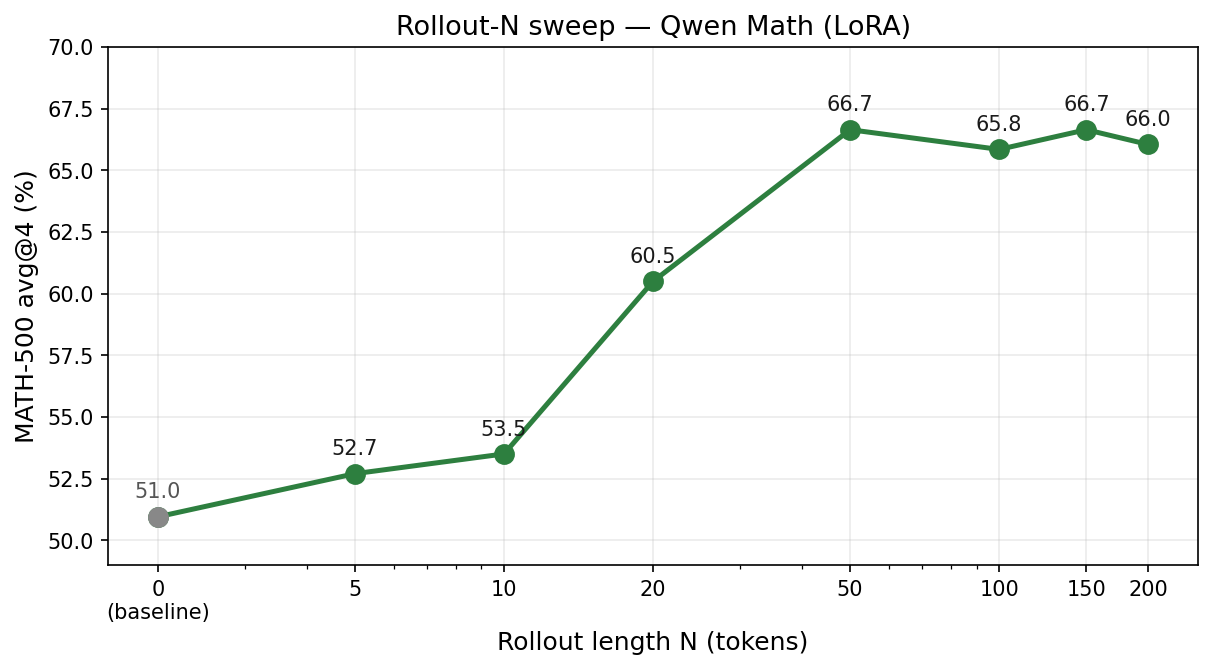
\includegraphics[width=0.65\linewidth]{figures/fig_n_sweep.png}
    \caption{\textbf{Rollout Length $N$ Sweep on MATH-500.} LoRA, Qwen2.5-Math-1.5B $\rightarrow$ Qwen3-1.7B; best avg@4 across training steps. Full rollout and the undistilled baseline are shown as horizontal references. Performance saturates for $N \in [50, 200]$ and all beat full-seq.}
    \label{fig:n_sweep}
\end{figure}


\subsection{Efficiency of \Method{}}
\label{sec:efficiency}

\begin{table}[t]
\centering
\small
\setlength{\tabcolsep}{4pt}
\begin{tabular}{lcccccc}
\toprule
& \multicolumn{3}{c}{\textit{Per-step wall time}} & \multicolumn{3}{c}{\textit{Peak GPU memory}} \\
\cmidrule(lr){2-4}\cmidrule(lr){5-7}
\textbf{Phase} & \textbf{\makecell{ESR\\(100 tok.)}} & \textbf{\makecell{Full\\rollout}} & \textbf{Speedup} & \textbf{\makecell{ESR\\(100 tok.)}} & \textbf{\makecell{Full\\rollout}} & \textbf{Savings} \\
\midrule
Teacher scoring     & 1\,s & 7\,s   & 7$\times$    & 7.3\,GB & 14.9\,GB & 2.0$\times$ \\
Student generation  & 5\,s & 180\,s & 36$\times$   & 7.2\,GB & 8.9\,GB  & 1.2$\times$ \\
Student training    & 2\,s & 7\,s   & 3.5$\times$  & 9.6\,GB & 39.5\,GB & 4.1$\times$ \\
\midrule
\textbf{Total (single step)} & \textbf{8\,s}    & \textbf{194\,s}   & \textbf{24$\times$} & \multirow{2}{*}{\textbf{24.1\,GB}} & \multirow{2}{*}{\textbf{63.3\,GB}} & \multirow{2}{*}{\textbf{2.6$\times$}} \\
\textbf{Total (200 steps)}   & \textbf{27\,min} & \textbf{10.8\,hr} & \textbf{24$\times$} & & & \\
\bottomrule
\end{tabular}
\caption{\textbf{Training efficiency.} Single A6000 (48\,GB), bs${=}16$, student teacher Qwen3-1.7B. We report the average running time and GPU memory usage across student model generation, training and teacher scoring phases. Note that the real time usage can be larger if there isn't enough GPU to hold the student and teacher models together and requires model loading and unloading.}
\label{tab:timing}
\end{table}

Table~\ref{tab:timing} shows that \method{} achieves a 24$\times$ wall-clock speedup and reduces peak training memory by $\sim 4\times$. The dominant cost in full-seq is autoregressive generation ($180$\,s/step for sequences averaging ${\sim}1000$ tokens); \method{} generates only $N{=}100$ tokens (5\,s/step). Note that with \method, all the student and teacher models can be put in one A6000 GPU comfortably. In our own practice, it saves a further big time overhead of model loading and unloading that we do not report here. 

% ============================================================================
% 6. MECHANISMS (Part 3 of the deck)
% ============================================================================
\section{Additional Reasons Why Does \Method{} Work? }
\label{sec:mechanisms_section}

The surprising effectiveness of \methodfull{} probes us to investigate deeper beyond what we have identified Section \ref{sec:motivation}. We structure this section around three questions: \textbf{(\S\ref{sec:token_selection})} Is the early-position effect induced by by high-KL or high-entropy tokens? \textbf{(\S\ref{sec:mechanisms})} If not, what additional structural reasons make the early window privileged? \textbf{(\S\ref{sec:mode_seek})} Why does \method{} sometimes \emph{exceed} the teacher?

\subsection{What Does The Effectiveness of \Method{} Stem From?}
\label{sec:token_selection}

In Section \ref{sec:motivation}, we identified the ``Off-policy Teacher Drift'' and ``Stale Late-position Lock-in'' problem that can cause the late-position tokens to provide degrading signals. During the experiment analysis, we find that, as shown in Figure~\ref{fig:three_curves}, early positions simultaneously have high KL divergence between student and teacher model, and high token entropy from both student and teacher models. This finding probes us to wonder if the effectiveness is intrinsically induced by the KL and entropy. To control these factors, we conduct a series of ablation experiments: pick the same amount (100) of tokens based on the highest KL divergence, highest student/teacher entropy or with them in combination with \method, regardless of position (Table~\ref{tab:token_select}). If the effectiveness is indeed induced by the KL or entropy, then they should reproduce the same or better results. 

\begin{figure}[t]
\centering
\begin{minipage}[b]{0.42\textwidth}
    \centering
    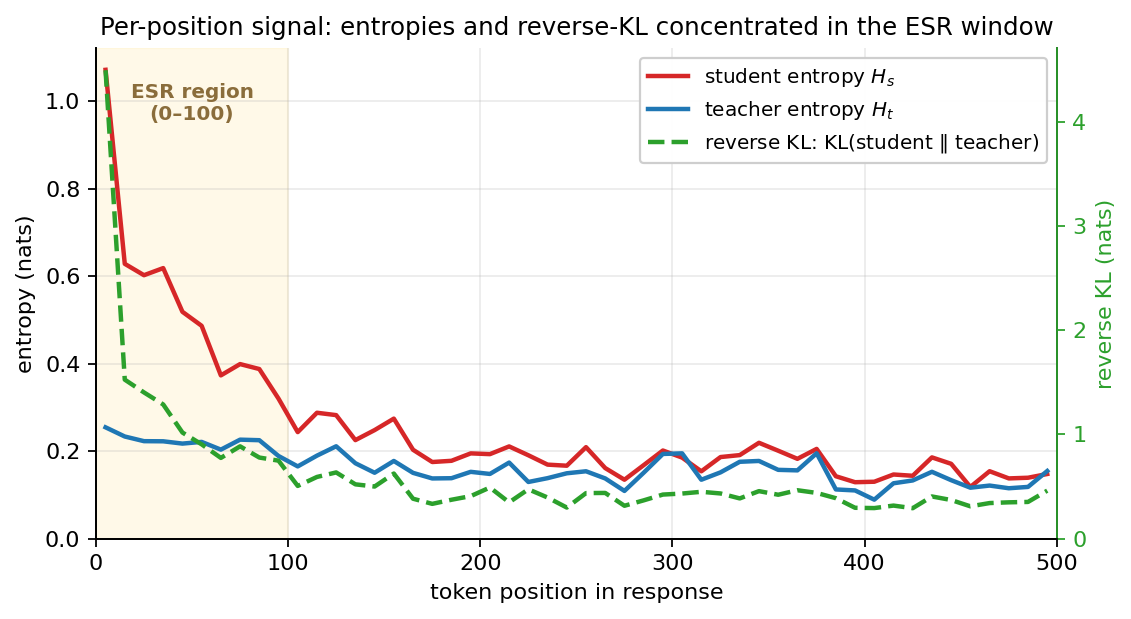
\includegraphics[width=\linewidth]{figures/three_curves_by_position.png}
    \captionof{figure}{\textbf{Early positions carry all three --- student entropy, teacher entropy, and reverse-KL --- simultaneously} (Qwen, MATH-500). Natural hypothesis: \method{} works because those regions carry the most signal (high KL) at the most uncertain points (high entropy). If that were the mechanism, selecting tokens by high-KL or high-entropy alone should recover the gain. Table~\ref{tab:token_select} shows it does not.}
    \label{fig:three_curves}
\end{minipage}
\hfill
\begin{minipage}[b]{0.55\textwidth}
    \centering
    \small
    \begin{tabular}{lcc}
    \toprule
    \textbf{Selection method} & \textbf{$k$} & \textbf{Best avg@4} \\
    \midrule
    \textbf{ESR-100 (ours)} & 100 & \textbf{65.85} \\
    Full-seq (all tokens) & --- & 62.35 \\
    \midrule
    Top-$\mathrm{RKL}$ & 100 & 53.35 \\
    Top-$H_t$ (teacher entropy) & 100 & 63.30 \\
    Top-$H_s$ (student entropy) & 100 & 62.70 \\
    Top-$H_s$ & 200 & 53.20 \\
    $\mathrm{RKL} \!\cdot\! H_s$ & 100 & 56.90 \\
    $H_t \!\cdot\! H_s$ (product) & 100 & 55.35 \\
    $\mathrm{RKL} \!\cdot\! H_t \!\cdot\! H_s$ (triple product) & 100 & 57.90 \\
    \bottomrule
    \end{tabular}
    \captionof{table}{\textbf{Token selection strategies on MATH-500.} Qwen2.5-Math-1.5B $\to$ Qwen3-1.7B, LoRA, $n_{\text{samples}}{=}1$, best avg@4 across training steps. All selectors operate on full-length rollouts; \method{} is the only one that additionally truncates the rollout. Baseline (no distillation) 50.95\%; full-seq 62.35\%. $H_s$: student entropy; $H_t$: teacher entropy; $\mathrm{RKL}$: reverse KL.}
    \label{tab:token_select}
\end{minipage}
\end{figure}

 To our surprise, all underperform \method{}, and most of them also much underperform the full rollout results. Teacher or student entropy based selection can match the full sequence by them alone, but their combination falls short significantly. What's also interesting is that KL divergence measure, the direct calculation of the loss magnitude, barely works. It only improves the baseline (50.95\%) for about 3 percent. And more surprisingly, we find that the largest 100 tokens of KL occupies around 93\% of the entire trajectory loss. This shows that the tokens that has larger signals are not necessarily the ones that have effective signals. 
 
 Therefore, althought we still don't exclude KL and entropy as potential mediator factor, we exclude them to be the sole factors that causes early tokens to be special. Position, therefore, should be considered an independent token selection dimension for the future.

\subsection{The Convergence Cascade Effect of \Method{}}
\label{sec:mechanisms}

We find an additional important mechanism that assists in \method's effectiveness. Even we only trained the first $N$ tokens with \method,  training, per-position KL divergence beyond $[0, N]$ region still drops  by $30$--$40\%$ (Figure~\ref{fig:cascade}). This shows that the student can pick up the teacher's ``global mindset'' even with just the beginning tokens. One reason that we suspect is that the beginning tokens often consist of problem framing and strategic planning content. Therefore once the student picks up how to frame problems and plan the strategy, the later content naturally follows.

Moreover, recently \cite{sublinminal} shows student models may be able to learn the teacher's deep internal preference even with random numbers generated by the teacher, called ``subliminal learning''. Therefore, the early tokens may suffice to inject the subliminal mindset to the student. 

\begin{figure}[t]
    \centering
    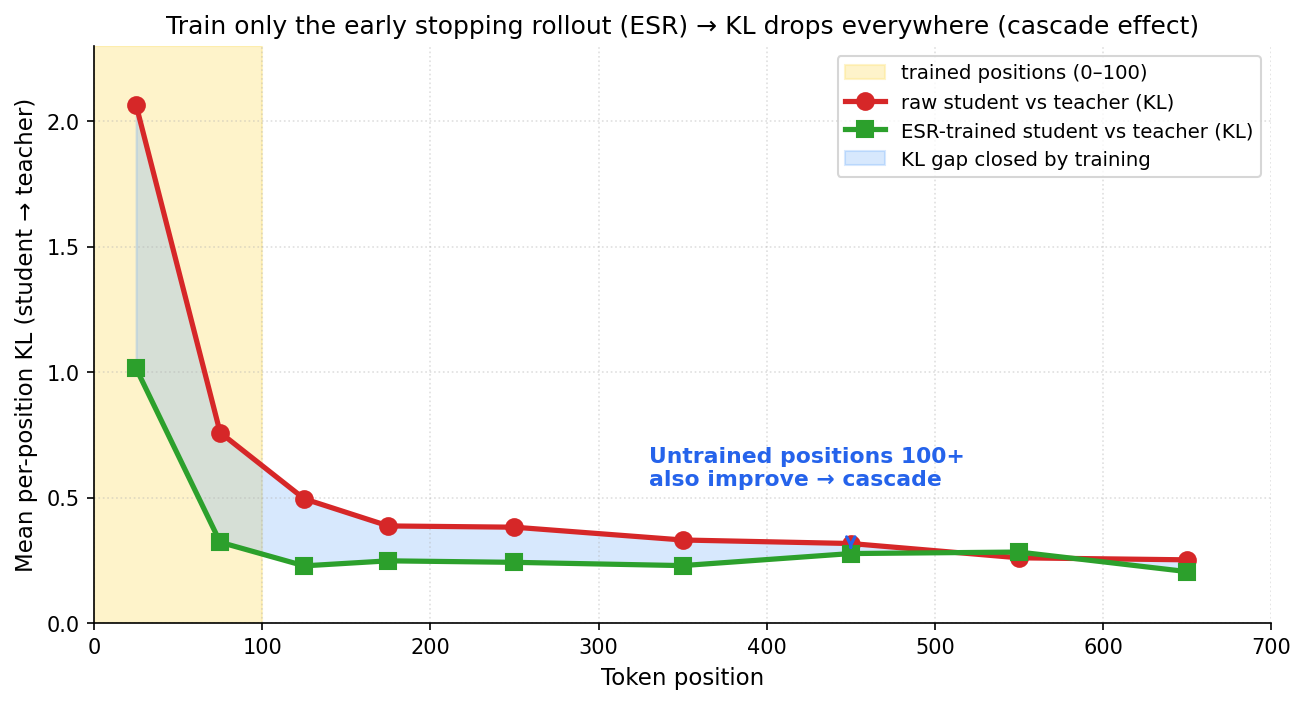
\includegraphics[width=0.85\linewidth]{figures/kl_cascade_curves.png}
    \caption{\textbf{The convergence cascade.} Per-position KL between distilled student and teacher, before vs.\ after \method training. Yellow band: positions $[0, 100]$ that actually receive training loss. Blue band: the KL gap closed by training. Positions $100+$ --- which see no direct training signal --- drop to the same KL as the trained region, confirming that alignment on the early window cascades through the autoregressive rollout.}
    \label{fig:cascade}
\end{figure}

\subsection{Why Does \Method{} Even Exceed the Teacher?}
\label{sec:mode_seek}

\Method{} exceeds the teacher on several cells (Qwen math; Qwen and Gemma function calling; Gemma coding, where the teacher is in fact weaker than the student). We offer a hypothesis. Reverse KL $\mathrm{KL}(\pi_s \,\|\, \pi_t)$ is mode-seeking: it penalizes the student for putting mass on tokens the teacher does not support, but not for concentrating mass on a single supported token. When the teacher is multi-modal at the planning positions---one mode being a verbose, wasteful plan and another a concise correct plan---a short early-window loss can force the student to commit to the smaller, correct mode rather than averaging (Figure~\ref{fig:mode_seek}). On function-calling this effect is pronounced: \method-100 lifts Qwen BFCL full\_acc from 54.0\% (teacher) to 61.3\%, and the chained Qwen3-4B$\to$8B configuration raises it to 76.8\% against a 73.0\% teacher. Full-sequence training cannot achieve this because its late-position loss pulls the student toward the average teacher behaviour across all supported modes, undoing the concentration.

\begin{figure}[t]
    \centering
    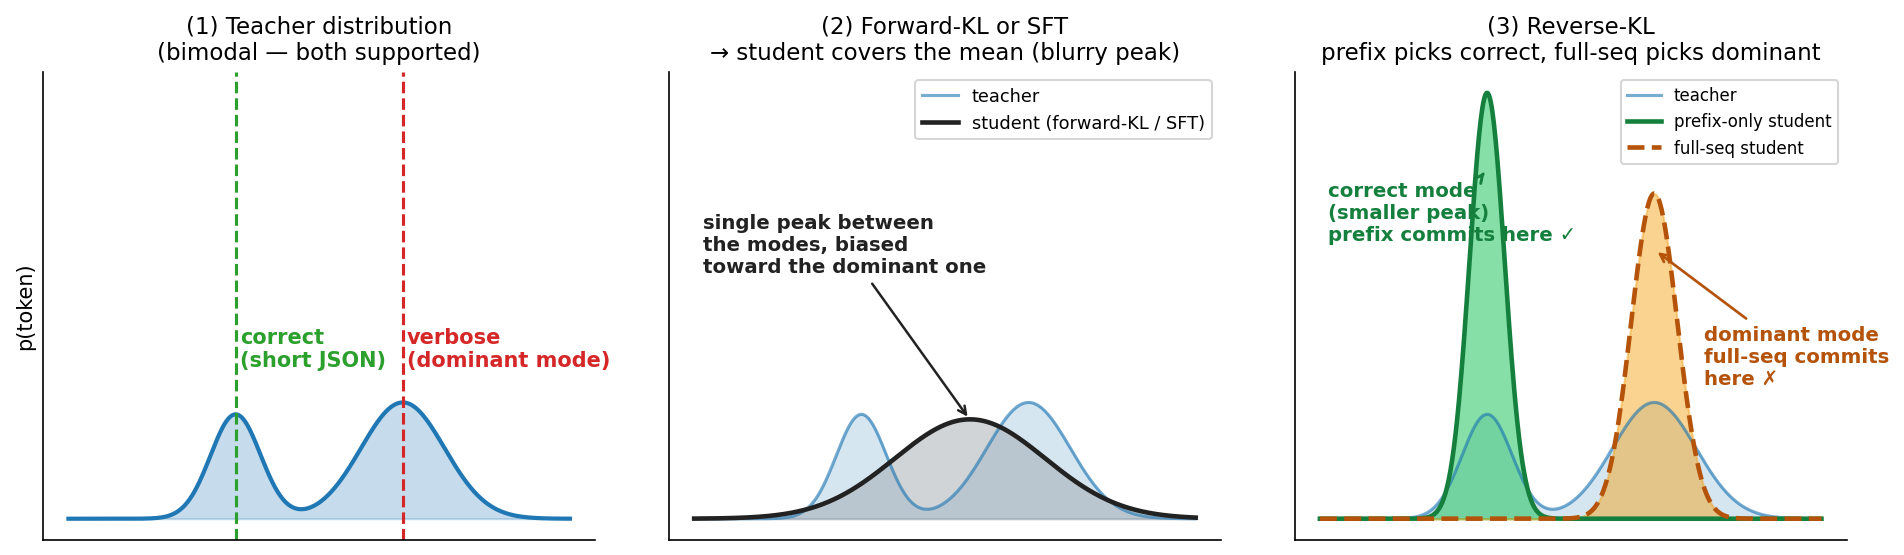
\includegraphics[width=0.85\linewidth]{figures/mode_seeking_schematic.png}
    \caption{\textbf{Mode-seeking on the planning region.} Schematic of reverse-KL behaviour at a multi-modal planning position. The teacher supports two modes (e.g.\ a verbose plan and a concise correct plan); reverse KL penalises student mass outside the support but not concentration within it. A short early-window loss can collapse the student onto the better supported mode, allowing the student to exceed the teacher's average behaviour. Full-sequence training reverts the student toward the averaged teacher across late positions, undoing the concentration.}
    \label{fig:mode_seek}
\end{figure}

\paragraph{Behavioral signature.} The hypothesis predicts that \method-trained students should (a) produce shorter, less-hedging rollouts than the teacher, and (b) commit hard, but on \emph{non-argmax} teacher modes. Table~\ref{tab:behavioral_signature} confirms both. \Method-100 rollouts are shorter than the base student, the teacher, \emph{and} full-seq across the entire length distribution --- even the top-decile ($\sim$800 tokens) is below the base student's median ($\sim$860). On the top-10\% highest-KL positions ($n{=}110{,}894$), \method{} raises student top-1 probability to $0.79$ (vs $0.77$ full-seq, $0.71$ base) while \emph{lowering} agreement with the teacher's argmax to $41.9\%$ (vs $45.7\%$ full-seq) and raising the rate at which the student picks tokens in the teacher's top-2 to top-5 to $47.4\%$ (vs $44.6\%$). \Method{} commits harder, but on different teacher-supported tokens; full-seq commits toward the teacher's argmax and inherits the teacher's mistakes on those positions.

\begin{table}[t]
\centering
\footnotesize
\setlength{\tabcolsep}{2.5pt}
\begin{tabular}{lccccc@{\hskip 5pt}cccc}
\toprule
& \multicolumn{5}{c}{\textbf{\makecell{Response length\\(tokens)}}} & \multicolumn{4}{c}{\textbf{\makecell{Student commitment\\\& mode alignment}}} \\
\cmidrule(lr){2-6}\cmidrule(lr){7-10}
\textbf{Model} & \textbf{\makecell{10th\\pctile}} & \textbf{\makecell{50th\\pctile}} & \textbf{\makecell{90th\\pctile}} & \textbf{Mean} & \textbf{Ratio} & \textbf{\makecell{Top-1\\prob}} & \textbf{\makecell{$=$ tch.\\top-1}} & \textbf{\makecell{$\in$ tch.\\top 2--5}} & \textbf{\makecell{$\notin$ tch.\\top-5}} \\
\midrule
Base student            & $\sim$400     & $\sim$860     & $\sim$1{,}500 & $\sim$990     & $2.2\times$ & 0.71          & 28.6\%           & 59.8\%          & 11.5\% \\
Teacher (Q3-1.7B)       & $\sim$700     & $\sim$1{,}150 & $\sim$1{,}800 & $\sim$1{,}210 & $2.6\times$ & ---           & ---              & ---             & ---    \\
Full-seq                & $\sim$1{,}190 & $\sim$1{,}530 & $\sim$1{,}770 & $\sim$1{,}480 & $3.2\times$ & 0.77          & \textbf{45.7\%}  & 44.6\%          & 9.7\%  \\
\textbf{\Method-100 (ours)} & $\sim$190 & $\sim$380     & $\sim$800     & $\sim$460     & $1.0\times$ & \textbf{0.79} & 41.9\%           & \textbf{47.4\%} & 10.7\% \\
\bottomrule
\end{tabular}
\caption{\textbf{Behavioral signature of \method{}.} \emph{Left:} Response length distribution on MATH-500 ($n{=}2{,}000$ rollouts per model; tokens estimated as $\text{chars}/3.5$). \Method-100 is shorter than base, teacher, \emph{and} full-seq across the whole distribution: even its long tail (90th pctile $\sim 800$ tok) is shorter than the base student's typical response (50th pctile $\sim 860$ tok). \textbf{Ratio} = mean length relative to \Method. Full-seq mean is below its median because length is clipped at \texttt{max\_new\_tokens}. \emph{Right:} Top-10\% of token positions ranked by KL$[\pi_s\,\|\,\pi_t]$ on 100 base-student trajectories ($n{=}110{,}894$). ``$=$ tch.\ top-1'', ``$\in$ tch.\ top 2--5'', and ``$\notin$ tch.\ top-5'' are mutually exclusive and sum to $100\%$ (teacher omitted because the comparison is student-vs-teacher). \Method-100 commits hardest (top-1 prob $0.79$) but agrees \emph{less} with the teacher's argmax than full-seq, and picks teacher-supported alternatives more often.}
\label{tab:behavioral_signature}
\end{table}

This is the mode-seeking mechanism in numbers. When one of those teacher-supported alternatives happens to be the correct mode, \method{} exceeds the teacher; full-seq cannot, because supervising the late tail pulls the student toward the teacher's argmax and the teacher's mistakes along with it. A full proof of this hypothesis is out of scope; we note only that it is the natural reverse-KL-mode-seeking story applied to the planning region, and that it is consistent with every surpass-teacher cell we observe.


% ============================================================================
% RELATED WORK
% ============================================================================
% =============================================================================
% related_work_section.tex --- Positional Distillation Paper
% Self-contained related work section (~0.75 page, shortened)
% Usage: % =============================================================================
% related_work_section.tex --- Positional Distillation Paper
% Self-contained related work section (~0.75 page, shortened)
% Usage: % =============================================================================
% related_work_section.tex --- Positional Distillation Paper
% Self-contained related work section (~0.75 page, shortened)
% Usage: \input{related_work_section.tex} in main.tex
% =============================================================================

\section{Related Work}
\label{sec:related_work}

\paragraph{Knowledge Distillation for Language Models.}
Knowledge distillation~\citep{hinton2015distilling,kim2016sequence} for autoregressive LLMs hinges on the choice of divergence and data distribution.
\citet{gu2024minillm} argued for reverse KL, and \citet{agarwal2024onpolicy} introduced on-policy GKD, which supervises student rollouts with teacher logits.
Subsequent work has explored skew KL with adaptive off-policy schedules~\citep{ko2024distillm}, generalized $f$-divergences~\citep{wen2023fdivergence}, mode- vs.\ mean-seeking dynamics~\citep{wu2025rethinking}, and speculative-decoding-style filtering~\citep{xu2025speculative}.
We build on the on-policy reverse-KL paradigm but ask an orthogonal question: holding divergence and data distribution fixed, \emph{which token positions along the student's rollout carry useful signal?}

\paragraph{Token-Level Importance in Distillation and Reasoning.}
Not all tokens contribute equally to learning.
\citet{wang2025beyond8020} showed that $\sim$20\% high-entropy ``forking tokens'' suffice for RL gradients; \citet{vassoyan2025ignorekl} relaxed KL on critical tokens to enable exploration; \citet{li2025preplan} identified a preplan-and-anchor mechanism in attention; and \citet{singh2026functional} pruned reasoning chains by functional importance.
In distillation specifically, recent work selects tokens via teacher verification~\citep{huang2025selectkd}, adaptive temperature~\citep{xie2026adakd}, student entropy along position/class/sample axes~\citep{tavor2026rethinking}, and entropy plus preference ranking~\citep{kim2026tsdkd}.
Our Section~\ref{sec:token_selection} ablation contradicts the shared premise: selecting tokens by top-KL, various top-entropy variants, or soft-weighted joint entropy all underperform \method{} and most underperform plain full-sequence training.
Position is the load-bearing axis; scalar saliencies are not.
This also reconciles \citet{wang2025beyond8020} with our findings: in on-policy distillation, high-entropy tokens are disproportionately concentrated in the uncontaminated early window.

\paragraph{Training Stability and Sequence Length.}
Full-sequence on-policy distillation is unstable: likelihood training degenerates into bland, repetitive text~\citep{holtzman2020curious}, and self-training drives model collapse~\citep{shumailov2024collapse}.
\citet{jang2026veto} proposed a geometric logit-space bridge to suppress harmful gradients on low-confidence tokens.
On the length axis, \citet{chen2025distillingessence} showed that supervised training on the first 50\% of tokens retains $\sim$91\% of full-sequence performance, and \citet{yan2026dasd} addressed exposure bias in long-CoT distillation via temperature scheduling.
Our approach is complementary: restricting the loss scope to early positions, where teacher--student agreement is naturally highest, yields stability through a simpler mechanism and eliminates the degenerate repetition unique to on-policy training.

\paragraph{Curriculum Learning.}
Curriculum learning~\citep{bengio2009curriculum} and scheduled sampling~\citep{bengio2015scheduled} gradually increase task difficulty.
For LLM pretraining, sequence-length warmup stabilizes training~\citep{li2022stability} and variable-length curricula accelerate convergence~\citep{pouransari2024dataset}.
Our progressive position schedule applies the curriculum principle to the distillation loss scope rather than to the input length---a form of curriculum specific to knowledge distillation.

\paragraph{Reasoning Distillation.}
Chain-of-thought prompting~\citep{wei2022chainofthought} made intermediate reasoning the unit of transfer, and DeepSeek-R1~\citep{deepseekr1} showed that SFT-distilling a strong reasoner into a smaller model is often competitive with direct RL.
On reasoning tasks (MATH-500, HumanEval/MBPP, BFCL) and a 1.5B-math-student $\to$ 8B-teacher sweep, \method{} surpasses the teacher on several cells, indicating that gains beyond the teacher are possible when the mode-seeking reverse-KL loss is restricted to the planning region---explaining why the on-policy, early-stopped-rollout regime is more efficient and stable than full-sequence on-policy distillation, which frequently degrades on coding and math.
 in main.tex
% =============================================================================

\section{Related Work}
\label{sec:related_work}

\paragraph{Knowledge Distillation for Language Models.}
Knowledge distillation~\citep{hinton2015distilling,kim2016sequence} for autoregressive LLMs hinges on the choice of divergence and data distribution.
\citet{gu2024minillm} argued for reverse KL, and \citet{agarwal2024onpolicy} introduced on-policy GKD, which supervises student rollouts with teacher logits.
Subsequent work has explored skew KL with adaptive off-policy schedules~\citep{ko2024distillm}, generalized $f$-divergences~\citep{wen2023fdivergence}, mode- vs.\ mean-seeking dynamics~\citep{wu2025rethinking}, and speculative-decoding-style filtering~\citep{xu2025speculative}.
We build on the on-policy reverse-KL paradigm but ask an orthogonal question: holding divergence and data distribution fixed, \emph{which token positions along the student's rollout carry useful signal?}

\paragraph{Token-Level Importance in Distillation and Reasoning.}
Not all tokens contribute equally to learning.
\citet{wang2025beyond8020} showed that $\sim$20\% high-entropy ``forking tokens'' suffice for RL gradients; \citet{vassoyan2025ignorekl} relaxed KL on critical tokens to enable exploration; \citet{li2025preplan} identified a preplan-and-anchor mechanism in attention; and \citet{singh2026functional} pruned reasoning chains by functional importance.
In distillation specifically, recent work selects tokens via teacher verification~\citep{huang2025selectkd}, adaptive temperature~\citep{xie2026adakd}, student entropy along position/class/sample axes~\citep{tavor2026rethinking}, and entropy plus preference ranking~\citep{kim2026tsdkd}.
Our Section~\ref{sec:token_selection} ablation contradicts the shared premise: selecting tokens by top-KL, various top-entropy variants, or soft-weighted joint entropy all underperform \method{} and most underperform plain full-sequence training.
Position is the load-bearing axis; scalar saliencies are not.
This also reconciles \citet{wang2025beyond8020} with our findings: in on-policy distillation, high-entropy tokens are disproportionately concentrated in the uncontaminated early window.

\paragraph{Training Stability and Sequence Length.}
Full-sequence on-policy distillation is unstable: likelihood training degenerates into bland, repetitive text~\citep{holtzman2020curious}, and self-training drives model collapse~\citep{shumailov2024collapse}.
\citet{jang2026veto} proposed a geometric logit-space bridge to suppress harmful gradients on low-confidence tokens.
On the length axis, \citet{chen2025distillingessence} showed that supervised training on the first 50\% of tokens retains $\sim$91\% of full-sequence performance, and \citet{yan2026dasd} addressed exposure bias in long-CoT distillation via temperature scheduling.
Our approach is complementary: restricting the loss scope to early positions, where teacher--student agreement is naturally highest, yields stability through a simpler mechanism and eliminates the degenerate repetition unique to on-policy training.

\paragraph{Curriculum Learning.}
Curriculum learning~\citep{bengio2009curriculum} and scheduled sampling~\citep{bengio2015scheduled} gradually increase task difficulty.
For LLM pretraining, sequence-length warmup stabilizes training~\citep{li2022stability} and variable-length curricula accelerate convergence~\citep{pouransari2024dataset}.
Our progressive position schedule applies the curriculum principle to the distillation loss scope rather than to the input length---a form of curriculum specific to knowledge distillation.

\paragraph{Reasoning Distillation.}
Chain-of-thought prompting~\citep{wei2022chainofthought} made intermediate reasoning the unit of transfer, and DeepSeek-R1~\citep{deepseekr1} showed that SFT-distilling a strong reasoner into a smaller model is often competitive with direct RL.
On reasoning tasks (MATH-500, HumanEval/MBPP, BFCL) and a 1.5B-math-student $\to$ 8B-teacher sweep, \method{} surpasses the teacher on several cells, indicating that gains beyond the teacher are possible when the mode-seeking reverse-KL loss is restricted to the planning region---explaining why the on-policy, early-stopped-rollout regime is more efficient and stable than full-sequence on-policy distillation, which frequently degrades on coding and math.
 in main.tex
% =============================================================================

\section{Related Work}
\label{sec:related_work}

\paragraph{Knowledge Distillation for Language Models.}
Knowledge distillation~\citep{hinton2015distilling,kim2016sequence} for autoregressive LLMs hinges on the choice of divergence and data distribution.
\citet{gu2024minillm} argued for reverse KL, and \citet{agarwal2024onpolicy} introduced on-policy GKD, which supervises student rollouts with teacher logits.
Subsequent work has explored skew KL with adaptive off-policy schedules~\citep{ko2024distillm}, generalized $f$-divergences~\citep{wen2023fdivergence}, mode- vs.\ mean-seeking dynamics~\citep{wu2025rethinking}, and speculative-decoding-style filtering~\citep{xu2025speculative}.
We build on the on-policy reverse-KL paradigm but ask an orthogonal question: holding divergence and data distribution fixed, \emph{which token positions along the student's rollout carry useful signal?}

\paragraph{Token-Level Importance in Distillation and Reasoning.}
Not all tokens contribute equally to learning.
\citet{wang2025beyond8020} showed that $\sim$20\% high-entropy ``forking tokens'' suffice for RL gradients; \citet{vassoyan2025ignorekl} relaxed KL on critical tokens to enable exploration; \citet{li2025preplan} identified a preplan-and-anchor mechanism in attention; and \citet{singh2026functional} pruned reasoning chains by functional importance.
In distillation specifically, recent work selects tokens via teacher verification~\citep{huang2025selectkd}, adaptive temperature~\citep{xie2026adakd}, student entropy along position/class/sample axes~\citep{tavor2026rethinking}, and entropy plus preference ranking~\citep{kim2026tsdkd}.
Our Section~\ref{sec:token_selection} ablation contradicts the shared premise: selecting tokens by top-KL, various top-entropy variants, or soft-weighted joint entropy all underperform \method{} and most underperform plain full-sequence training.
Position is the load-bearing axis; scalar saliencies are not.
This also reconciles \citet{wang2025beyond8020} with our findings: in on-policy distillation, high-entropy tokens are disproportionately concentrated in the uncontaminated early window.

\paragraph{Training Stability and Sequence Length.}
Full-sequence on-policy distillation is unstable: likelihood training degenerates into bland, repetitive text~\citep{holtzman2020curious}, and self-training drives model collapse~\citep{shumailov2024collapse}.
\citet{jang2026veto} proposed a geometric logit-space bridge to suppress harmful gradients on low-confidence tokens.
On the length axis, \citet{chen2025distillingessence} showed that supervised training on the first 50\% of tokens retains $\sim$91\% of full-sequence performance, and \citet{yan2026dasd} addressed exposure bias in long-CoT distillation via temperature scheduling.
Our approach is complementary: restricting the loss scope to early positions, where teacher--student agreement is naturally highest, yields stability through a simpler mechanism and eliminates the degenerate repetition unique to on-policy training.

\paragraph{Curriculum Learning.}
Curriculum learning~\citep{bengio2009curriculum} and scheduled sampling~\citep{bengio2015scheduled} gradually increase task difficulty.
For LLM pretraining, sequence-length warmup stabilizes training~\citep{li2022stability} and variable-length curricula accelerate convergence~\citep{pouransari2024dataset}.
Our progressive position schedule applies the curriculum principle to the distillation loss scope rather than to the input length---a form of curriculum specific to knowledge distillation.

\paragraph{Reasoning Distillation.}
Chain-of-thought prompting~\citep{wei2022chainofthought} made intermediate reasoning the unit of transfer, and DeepSeek-R1~\citep{deepseekr1} showed that SFT-distilling a strong reasoner into a smaller model is often competitive with direct RL.
On reasoning tasks (MATH-500, HumanEval/MBPP, BFCL) and a 1.5B-math-student $\to$ 8B-teacher sweep, \method{} surpasses the teacher on several cells, indicating that gains beyond the teacher are possible when the mode-seeking reverse-KL loss is restricted to the planning region---explaining why the on-policy, early-stopped-rollout regime is more efficient and stable than full-sequence on-policy distillation, which frequently degrades on coding and math.



% ============================================================================
% CONCLUSION
% ============================================================================
\section{Conclusion}
\label{sec:conclusion}

In on-policy knowledge distillation, the teacher's per-token supervision quality is a strong, monotonic function of position: early tokens carry strong, independent signal about reasoning strategy; late tokens, scored on the student's own contaminated previous output, contribute weak, dependent signal that is actively harmful when trained on. A one-line intervention --- restrict the loss and the rollout to the first $N$ response tokens --- yields four simultaneous wins: (i) \textbf{better}, matching or exceeding full-sequence distillation on every task/family/regime we test and surpassing the teacher in nine cells; (ii) \textbf{faster}, $20$--$35\times$ wall-clock with $4\times$ less GPU memory; (iii) \textbf{stabler}, eliminating HumanEval collapse, BFCL parse-rate collapse, and the MATH-500 boxed-repetition failure mode; and (iv) \textbf{structural}, in that selecting the same number of tokens by any KL or entropy saliency fails --- position is an independent axis, not a proxy for scalar surprise. Teaching the student how to begin is sufficient to improve the entire response.

\paragraph{Limitations.} Our experiments are conducted on small open-source models with a limited data budget; whether the \method{} story holds at industrial scale (much larger students, teachers, and training corpora) remains unclear. We also do not test multi-modality or long-horizon tasks, both of which may exhibit different positional signal-quality patterns.


% ============================================================================
% ACKNOWLEDGMENTS
% ============================================================================
% The `ack` environment is automatically hidden in the anonymized submission
% and shown only in `final` / `preprint` compilations.
\begin{ack}
Funding and competing-interest disclosures will appear here in the final
version. See \url{https://neurips.cc/Conferences/2026/PaperInformation/FundingDisclosure}.
\end{ack}


% ============================================================================
% REFERENCES
% ============================================================================
\bibliographystyle{plainnat}
\bibliography{references_extended}


% ============================================================================
% APPENDIX
% ============================================================================
\appendix

\section{Training Efficiency}
\label{app:timing}

\begin{table}[!htbp]
\centering
\caption{\textbf{Training efficiency, detailed breakdown.} Per-step wall-clock time on a single A6000 (48GB). Student: Qwen2.5-Math-1.5B, LoRA, bs=16.}
\label{tab:timing_detail}
\small
\begin{tabular}{llcccc}
\toprule
\textbf{Teacher} & \textbf{Method} & \textbf{Gen (s)} & \textbf{Score (s)} & \textbf{Train (s)} & \textbf{Total (s)} \\
\midrule
\multirow{2}{*}{Q3-1.7B} & Full-seq & 100--731 & 3--10 & 5--12 & ${\sim}$280 \\
 & Ours ($N{=}100$) & ${\sim}$5 & ${\sim}$1 & ${\sim}$2 & ${\sim}$8 \\
\midrule
\multirow{2}{*}{Q3-4B} & Full-seq & 97--733 & 3--9 & 6--10 & ${\sim}$210 \\
 & Ours ($N{=}100$) & ${\sim}$5 & ${\sim}$1 & ${\sim}$2 & ${\sim}$8 \\
\midrule
\multirow{2}{*}{Q3-8B} & Full-seq & 96--230 & 7--11 & 1--6 & ${\sim}$170$^\dagger$ \\
 & Ours ($N{=}100$) & ${\sim}$5 & ${\sim}$1 & ${\sim}$2 & ${\sim}$8 \\
\bottomrule
\multicolumn{6}{l}{\footnotesize $^\dagger$ Frequent OOMs; 48GB insufficient for 8B teacher + vLLM + student.}
\end{tabular}
\end{table}


\section{Additional Student-Teacher Pairs}
\label{app:additional_pairs}

\begin{table}[!htbp]
\centering
\caption{\textbf{Additional student-teacher pairs.} All use ESR-100, LoRA, 3,200 problems.}
\label{tab:additional_pairs}
\small
\begin{tabular}{llccc}
\toprule
\textbf{Student} & \textbf{Teacher} & \textbf{MATH-500 avg@4} & \textbf{BFCL full\_acc} & \textbf{HumanEval pass@1} \\
\midrule
Qwen3-1.7B & --- (baseline) & 69.20\% & 59.80\% & 39.63\% \\
Qwen3-1.7B & Qwen3-4B & 69.20\% & 73.70\% & 44.51\% \\
Qwen3-1.7B & Qwen3-8B & 69.15\% & 74.00\% & 40.24\% \\
\midrule
Qwen3-4B & --- (baseline) & 77.95\% & 73.00\% & 73.17\% \\
Qwen3-4B & Qwen3-8B & 77.05\% & 76.80\% & 71.34\% \\
\bottomrule
\end{tabular}
\end{table}


\section{Full Experimental Results}
\label{app:full_results}

\subsection{Math Results: Per-Step Performance}

Table~\ref{tab:app_math_main} presents per-step results for the primary math experiments (LoRA, $n{=}1$, 3,200 problems).

\begin{table}[!htbp]
\centering
\caption{\textbf{MATH-500 per-step results.} LoRA, $n{=}1$, $\text{bs}{=}16$, 3,200 problems. Baseline: 50.95\% avg@4.}
\label{tab:app_math_main}
\small
\begin{tabular}{ll cccc}
\toprule
\textbf{Method} & \textbf{Metric} & \textbf{Step 50} & \textbf{Step 100} & \textbf{Step 150} & \textbf{Step 200} \\
\midrule
\multirow{3}{*}{ESR-50} & avg@4 & 62.35 & 66.05 & \textbf{66.65} & 64.85 \\
 & maj@4 & 69.40 & 72.00 & 71.00 & 71.20 \\
 & pass@4 & 77.20 & 79.40 & 81.00 & 79.60 \\
\midrule
\multirow{3}{*}{ESR-100} & avg@4 & 63.75 & 64.45 & 65.15 & \textbf{65.85} \\
 & maj@4 & 70.00 & 68.40 & 69.60 & 70.80 \\
 & pass@4 & 79.80 & 78.40 & 80.20 & 79.80 \\
\midrule
\multirow{3}{*}{ESR-150} & avg@4 & 65.35 & \textbf{66.65} & 65.30 & 65.75 \\
 & maj@4 & 66.80 & 67.00 & 66.30 & 67.30 \\
 & pass@4 & 79.00 & 81.00 & 78.20 & 80.00 \\
\midrule
\multirow{3}{*}{ESR-200} & avg@4 & \textbf{66.05} & 64.65 & 65.10 & 65.55 \\
 & maj@4 & 71.20 & 68.40 & 70.00 & 71.20 \\
 & pass@4 & 81.00 & 79.80 & 80.60 & 80.60 \\
\bottomrule
\end{tabular}
\end{table}


\subsection{Math Results: Earlier Series ($n{=}16$, 200 problems)}

\begin{table}[!htbp]
\centering
\caption{\textbf{Complete MATH-500 results, LoRA, $n{=}16$, $\text{bs}{=}16$.} Best per configuration in \textbf{bold}.}
\label{tab:app_math_n16}
\footnotesize
\begin{tabular}{lcccc}
\toprule
\textbf{Config} & \textbf{Step 50} & \textbf{Step 100} & \textbf{Step 150} & \textbf{Step 200} \\
\midrule
\multicolumn{5}{l}{\textit{avg@4}} \\
\midrule
ESR-5 & 55.15 & 55.65 & \textbf{56.50} & 56.30 \\
ESR-10 & \textbf{59.50} & 56.40 & 56.30 & 56.00 \\
ESR-20 & \textbf{60.20} & 57.35 & 56.40 & 56.55 \\
ESR-50 & \textbf{62.45} & 62.15 & 60.50 & 61.90 \\
ESR-100 & 61.15 & 63.55 & \textbf{64.25} & 63.85 \\
ESR-150 & 63.55 & \textbf{65.70} & 64.80 & 64.40 \\
ESR-200 & 63.25 & \textbf{66.75} & 64.55 & 65.25 \\
Progressive & 61.10 & 62.05 & 61.95 & \textbf{62.30} \\
Full-seq$^\dagger$ & \textbf{65.60} & 46.30 & 49.70 & 43.80 \\
Full-seq (first-boxed) & \textbf{65.55} & 64.95 & 65.55 & 64.95 \\
\midrule
\multicolumn{5}{l}{\textit{pass@4}} \\
\midrule
ESR-5 & 74.0 & 74.8 & \textbf{76.0} & 73.4 \\
ESR-10 & \textbf{75.8} & 73.2 & 75.4 & 74.2 \\
ESR-20 & \textbf{77.0} & 76.0 & 73.4 & 75.8 \\
ESR-50 & 77.0 & 78.4 & 77.6 & \textbf{78.6} \\
ESR-100 & 77.6 & 79.2 & \textbf{80.2} & 80.2 \\
ESR-150 & 79.6 & 77.4 & \textbf{80.0} & 79.4 \\
ESR-200 & 79.6 & \textbf{80.2} & 79.4 & 79.2 \\
Progressive & 77.2 & 77.8 & 78.2 & \textbf{78.8} \\
Full-seq & \textbf{80.0} & 72.2 & 77.0 & 74.2 \\
\bottomrule
\multicolumn{5}{l}{\footnotesize $^\dagger$ Last-boxed extraction; degrades due to repetition.}
\end{tabular}
\end{table}


\subsection{Coding Results}

\begin{table}[!htbp]
\centering
\caption{\textbf{Complete coding results, LoRA.} HumanEval (HE) and MBPP pass@1.}
\label{tab:app_coding_lora}
\footnotesize
\begin{tabular}{llcccccccc}
\toprule
\textbf{Config} & \textbf{Metric} & \textbf{s50} & \textbf{s100} & \textbf{s150} & \textbf{s200} & \textbf{s250} & \textbf{s300} & \textbf{s350} & \textbf{s400} \\
\midrule
\multirow{2}{*}{ESR-50} & HE & 37.8 & 39.0 & 39.6 & 41.5 & 40.2 & 40.9 & \textbf{42.1} & 40.9 \\
 & MBPP & 52.1 & 48.9 & 46.0 & 46.0 & 47.6 & 46.3 & 46.6 & 46.3 \\
\midrule
\multirow{2}{*}{ESR-100} & HE & 37.2 & 39.0 & \textbf{42.1} & 37.8 & 39.0 & 37.8 & 37.8 & 38.4 \\
 & MBPP & 52.1 & 49.7 & 49.2 & 49.2 & 48.4 & 49.2 & 47.9 & 48.9 \\
\midrule
\multirow{2}{*}{ESR-150} & HE & 36.6 & 35.4 & 36.6 & 39.0 & \textbf{41.5} & 39.6 & 38.4 & 37.2 \\
 & MBPP & 51.3 & 50.0 & 48.4 & 50.5 & 49.5 & 50.3 & 49.7 & 48.7 \\
\midrule
\multirow{2}{*}{Full-seq} & HE & \textbf{40.2} & 31.7 & 32.3 & 32.9 & 27.4 & 28.0 & 26.8 & 26.8 \\
 & MBPP & 52.6 & 48.9 & 49.5 & 48.1 & 47.9 & 47.1 & 48.4 & 47.6 \\
\bottomrule
\end{tabular}
\end{table}


\subsection{Function Calling Results}

\begin{table}[!htbp]
\centering
\caption{\textbf{Function calling results (BFCL), LoRA.} Name accuracy / Full accuracy / Parse rate. Best full\_acc in \textbf{bold}.}
\label{tab:app_funcall}
\small
\begin{tabular}{lccccc}
\toprule
\textbf{Method} & \textbf{Best Step} & \textbf{Name Acc} & \textbf{Full Acc} & \textbf{Parse Rate} \\
\midrule
Baseline & --- & 9.70\% & 2.70\% & 24.20\% \\
Teacher (Qwen3-1.7B) & --- & 75.30\% & 54.00\% & 75.30\% \\
\midrule
ESR-50 & 200 & 95.20\% & 57.20\% & 98.30\% \\
\textbf{ESR-100} & \textbf{100} & 86.20\% & \textbf{61.30\%} & 91.30\% \\
ESR-150 & 200 & 88.70\% & 61.50\% & 92.50\% \\
ESR-200 & 200 & 80.80\% & 54.50\% & 90.20\% \\
Full-seq & 100 & 81.00\% & 58.20\% & 86.70\% \\
\bottomrule
\end{tabular}
\end{table}


\subsection{Scaling Experiment Results}

\begin{table}[!htbp]
\centering
\caption{\textbf{Scaling results.} All use ESR-100, LoRA, 3,200 problems. Best across training steps. Baseline performance shown for reference.}
\label{tab:app_scaling}
\small
\begin{tabular}{llccc}
\toprule
\textbf{Student $\rightarrow$ Teacher} & \textbf{Math avg@4} & \textbf{BFCL full\_acc} & \textbf{HE pass@1} & \textbf{MBPP+ pass@1} \\
\midrule
M-1.5B baseline & 50.95\% & 2.70\% & --- & --- \\
M-1.5B $\rightarrow$ Q3-1.7B & 65.85\% & 61.30\% & 42.07\% & 44.44\% \\
M-1.5B $\rightarrow$ Q3-4B & 68.95\% & 45.80\% & 43.29\% & 47.62\% \\
M-1.5B $\rightarrow$ Q3-8B & 67.85\% & 57.00\% & 41.46\% & 44.44\% \\
\midrule
Q3-1.7B baseline & 69.20\% & 59.80\% & 39.63\% & 44.71\% \\
Q3-1.7B $\rightarrow$ Q3-4B & 69.20\% & 73.70\% & 44.51\% & 47.62\% \\
Q3-1.7B $\rightarrow$ Q3-8B & 69.15\% & 74.00\% & 40.24\% & 48.15\% \\
\midrule
Q3-4B baseline & 77.95\% & 73.00\% & 73.17\% & 55.56\% \\
Q3-4B $\rightarrow$ Q3-8B & 77.05\% & 76.80\% & 71.34\% & 56.35\% \\
\bottomrule
\end{tabular}
\end{table}


\subsection{Full-Sequence Degradation Details}
\label{app:fullseq_degradation}

Table~\ref{tab:app_fullseq_collapse} summarises every full-rollout cell (across pairs, tasks, and regimes) for which we have a per-step trajectory on disk and observe degradation across training. For each cell we report the \emph{peak} score (best checkpoint across training) and the \emph{lowest} score (worst checkpoint after the peak), together with the step indices at which they occur. Bold $\Delta$ values indicate cells where Full Rollout drops below the student baseline. The Qwen-math \mbox{$n{=}16$} row (boxed-repetition collapse) is documented in greater detail in Table~\ref{tab:app_boxed} below.

\begin{table}[!htbp]
\centering
\caption{\textbf{Full-rollout collapses across training (peak $\rightarrow$ lowest).} Each row is a single Full Rollout experiment; we report the highest and lowest checkpoint scores across all saved steps. ``$\Delta$'' is lowest $-$ peak. Cells with $^{\dagger}$ end the run \emph{below the student baseline}. Trajectories are taken from the per-step eval logs on the training cluster (\texttt{docs/main\_results.md}, \texttt{docs/scaling\_results.md}). \method{} on the same cells (not shown here) stays within $\pm$1pp of its peak across training; see Tables~\ref{tab:app_math_main} and~\ref{tab:app_coding_lora}.}
\label{tab:app_fullseq_collapse}
\footnotesize
\begin{tabular}{llllccc}
\toprule
\textbf{Pair} & \textbf{Regime} & \textbf{Task} & \textbf{Metric} & \textbf{Peak (step)} & \textbf{Lowest (step)} & \textbf{$\Delta$} \\
\midrule
Qwen-1.5B $\rightarrow$ Q3-1.7B & LoRA   & MATH-500 ($n{=}16$) & avg@4   & 65.60 (s50)  & 43.80 (s200)$^{\dagger}$ & $\mathbf{-21.80}$ \\
Qwen-1.5B $\rightarrow$ Q3-4B   & LoRA   & MATH-500            & avg@4   & 67.45 (s50)  & 54.45 (s100)             & $-13.00$ \\
Qwen-1.5B $\rightarrow$ Q3-4B   & LoRA   & MATH-500            & maj@4   & 73.20 (s50)  & 63.40 (s200)             & $-9.80$  \\
\midrule
Qwen-1.5B $\rightarrow$ Q3-1.7B & LoRA   & HumanEval           & pass@1  & 40.2 (s50)   & 26.8 (s350)              & $-13.4$ \\
Qwen-1.5B $\rightarrow$ Q3-1.7B & LoRA   & HumanEval+          & pass@1  & 35.4 (s50)   & 25.0 (s250)              & $-10.4$ \\
Qwen-1.5B $\rightarrow$ Q3-1.7B & FullFT & HumanEval           & pass@1  & 36.6 (s150)  & 30.5 (s300)              & $-6.1$  \\
Qwen-1.5B $\rightarrow$ Q3-1.7B & FullFT & HumanEval+          & pass@1  & 31.7 (s150)  & 26.2 (s250)              & $-5.5$  \\
Gemma-2-2B $\rightarrow$ Gemma-3-4B & LoRA & HumanEval         & pass@1  & 22.0 (s50)   & 11.6 (s150)$^{\dagger}$  & $\mathbf{-10.4}$ \\
\bottomrule
\multicolumn{7}{l}{\footnotesize $^{\dagger}$ Lowest score is below the student baseline (Qwen-Math-1.5B MATH-500: 50.95\%; Gemma-2-2B HumanEval: 23.78\%).}
\end{tabular}
\end{table}

\paragraph{Per-step trajectories} for the seven cells in Table~\ref{tab:app_fullseq_collapse}:

\begin{itemize}
\item \textbf{Qwen-1.5B$\rightarrow$Q3-1.7B, LoRA, HumanEval (pass@1):}
40.2 (s50) $\rightarrow$ 31.7 $\rightarrow$ 32.3 $\rightarrow$ 32.9 $\rightarrow$ 27.4 $\rightarrow$ 28.0 $\rightarrow$ 26.8 $\rightarrow$ 26.8 (s400).
\item \textbf{Qwen-1.5B$\rightarrow$Q3-1.7B, LoRA, HumanEval+ (pass@1):}
35.4 (s50) $\rightarrow$ 27.4 $\rightarrow$ 29.9 $\rightarrow$ 29.9 $\rightarrow$ 25.0 $\rightarrow$ 26.2 $\rightarrow$ 25.0 $\rightarrow$ 25.0 (s400).
\item \textbf{Qwen-1.5B$\rightarrow$Q3-1.7B, FullFT, HumanEval (pass@1):}
32.3 $\rightarrow$ 32.3 $\rightarrow$ 36.6 (s150) $\rightarrow$ 36.0 $\rightarrow$ 31.1 $\rightarrow$ 30.5 $\rightarrow$ 31.7 $\rightarrow$ 31.1 (s400).
\item \textbf{Qwen-1.5B$\rightarrow$Q3-1.7B, FullFT, HumanEval+ (pass@1):}
27.4 $\rightarrow$ 28.7 $\rightarrow$ 31.7 (s150) $\rightarrow$ 30.5 $\rightarrow$ 26.2 $\rightarrow$ 26.2 $\rightarrow$ 26.8 $\rightarrow$ 26.2 (s400).
\item \textbf{Gemma-2-2B$\rightarrow$Gemma-3-4B, LoRA, HumanEval (pass@1):}
22.0 (s50) $\rightarrow$ 14.6 $\rightarrow$ 11.6 $\rightarrow$ 11.6 (s200). Falls below the 23.78 student baseline at s100 and stays there.
\item \textbf{Qwen-1.5B$\rightarrow$Q3-4B, LoRA, MATH-500 avg@4:}
67.45 (s50) $\rightarrow$ 54.45 $\rightarrow$ 58.85 $\rightarrow$ 55.05 (s200) (boxed-repetition pattern; \method{}-100 on the same pair climbs to 68.95).
\item \textbf{Qwen-1.5B$\rightarrow$Q3-1.7B, LoRA, MATH-500 ($n{=}16$) avg@4:}
65.60 (s50) $\rightarrow$ 46.30 $\rightarrow$ 49.70 $\rightarrow$ 43.80 (s200). Boxed-repetition collapse; statistics in Table~\ref{tab:app_boxed}.
\end{itemize}

\begin{table}[!htbp]
\centering
\caption{\textbf{Boxed repetition progression} in full-sequence LoRA distillation on MATH-500 ($n{=}16$, $\text{bs}{=}16$). Companion to the corresponding row of Table~\ref{tab:app_fullseq_collapse}.}
\label{tab:app_boxed}
\small
\begin{tabular}{lcccc}
\toprule
\textbf{Statistic} & \textbf{Step 50} & \textbf{Step 100} & \textbf{Step 150} & \textbf{Step 200} \\
\midrule
Multi-boxed responses & 2.9\% & 91.5\% & 80.5\% & 89.1\% \\
Avg \bboxed{} per response & 1.0 & 88.1 & 54.1 & 58.0 \\
Repetitive responses & 5.9\% & 78.8\% & 58.3\% & 77.5\% \\
Avg response length (chars) & 1,388 & 4,023 & 3,585 & 4,558 \\
\midrule
Official avg@4 & 65.60\% & 46.30\% & 49.70\% & 43.80\% \\
Relaxed avg@4 (GT in text) & 74.60\% & 70.90\% & 71.90\% & 70.30\% \\
\bottomrule
\end{tabular}
\end{table}


\section{KL-Profile Diagnostic for Choosing $N$}
\label{app:kl_profile}

A practical question for a new student--teacher pair is: what value of $N$ should I use? Our position-sweep (Section~\ref{sec:stability}) shows a wide plateau on Qwen math ($N \in [50, 200]$, avg@4 within $\sim$1pp); the same plateau appears on Gemma math ($N \approx 100$). These plateau locations coincide with the position at which the cumulative per-position KL $\sum_{k \le N} \mathbb{E}[\KL_k]$ reaches $\sim$45\% of the full-trajectory total, measured on a small ($\sim$1k trajectory) pre-training rollout. This suggests a cheap rule of thumb: run a 1k-trajectory per-position KL scan before training, and pick $N$ at the 45\% cumulative-KL point. We verify this on two cells (Qwen, Gemma math) and leave a full six-cell verification ($\{$Qwen, Gemma$\}\times\{$math, coding, funcall$\}$) as a short follow-up (\tbd{KL-profile scan}); the diagnostic is reported here as a practical recipe rather than a claim.

\section{Token Classification Methodology}
\label{app:token_classification}

We classify each token into six categories based on string matching:
\begin{enumerate}
    \item \textbf{planning}: Reasoning keywords (``To'', ``Let'', ``First'', ``Step'', ``We'', ``Given'', ``Therefore'', ``Thus'', ``Since'').
    \item \textbf{structural}: Punctuation, whitespace, formatting tokens.
    \item \textbf{math\_number}: Digits (0--9).
    \item \textbf{math\_operator}: Arithmetic operators ($+$, $-$, $\times$, $/$, $=$).
    \item \textbf{math\_latex}: LaTeX delimiters (\texttt{\textbackslash(}, \texttt{\textbackslash[}).
    \item \textbf{continuation}: All others.
\end{enumerate}

\begin{table}[!htbp]
\centering
\caption{\textbf{Mean KL by token category and position range.}}
\label{tab:app_kl_by_category}
\small
\begin{tabular}{lcccccc}
\toprule
\textbf{Category} & \textbf{0--4} & \textbf{5--19} & \textbf{20--49} & \textbf{50--99} & \textbf{100--199} & \textbf{200--499} \\
\midrule
planning & 4.50 & 0.79 & 1.49 & 1.66 & 1.49 & 2.37 \\
structural & 3.26 & 1.46 & 1.60 & 0.93 & 0.60 & 0.86 \\
math\_number & 1.49 & 0.60 & 0.74 & 0.28 & 0.17 & 0.13 \\
math\_operator & 7.30 & 1.84 & 0.81 & 0.37 & 0.21 & 0.14 \\
math\_latex & 8.84 & 9.23 & 6.50 & 4.95 & 2.97 & 1.87 \\
continuation & 1.94 & 1.12 & 1.19 & 0.89 & 0.70 & 0.48 \\
\bottomrule
\end{tabular}
\end{table}

\begin{table}[!htbp]
\centering
\caption{\textbf{Top 20 highest-KL tokens} (minimum 50 occurrences across 10,000 trajectories).}
\label{tab:app_high_kl_tokens}
\small
\begin{tabular}{clccc}
\toprule
\textbf{Rank} & \textbf{Token} & \textbf{Category} & \textbf{Count} & \textbf{Mean KL} \\
\midrule
1 & ``Solution'' & planning & 152 & 21.93 \\
2 & ``Analysis'' & continuation & 125 & 16.49 \\
3 & \texttt{\textbackslash[} & math\_latex & 7,152 & 13.21 \\
4 & ``examines'' & continuation & 74 & 11.51 \\
5 & ``He'' & continuation & 150 & 10.80 \\
6 & \texttt{\textbackslash(} & math\_latex & 21,243 & 10.30 \\
7 & ``First'' & planning & 1,706 & 9.98 \\
8 & ``tests'' & continuation & 52 & 8.71 \\
9 & \texttt{\textbackslash\textbackslash} & math\_latex & 82 & 8.68 \\
10 & ``There'' & continuation & 201 & 8.28 \\
11 & ``Therefore'' & planning & 4,913 & 7.95 \\
12 & ``Identify'' & continuation & 1,345 & 7.78 \\
13 & ``To'' & planning & 8,806 & 6.90 \\
14 & ``When'' & continuation & 89 & 6.62 \\
15 & ``This'' & continuation & 621 & 6.34 \\
16 & ``Thus'' & planning & 2,547 & 6.24 \\
17 & ``First'' (space) & planning & 259 & 6.10 \\
18 & ``To'' (space) & planning & 1,174 & 5.37 \\
19 & ``The'' & planning & 2,626 & 5.25 \\
20 & ``Next'' & planning & 1,753 & 5.03 \\
\bottomrule
\end{tabular}
\end{table}


% ============================================================================
% NEURIPS PAPER CHECKLIST (required, does not count toward page limit)
% ============================================================================
\newpage
\section*{NeurIPS Paper Checklist}

\begin{enumerate}

\item {\bf Claims}
    \item[] Question: Do the main claims made in the abstract and introduction accurately reflect the paper's contributions and scope?
    \item[] Answer: \answerYes{}
    \item[] Justification: The abstract and \S\ref{sec:intro} state that ESR matches or exceeds full-rollout distillation while being $20$--$35\times$ faster with $\sim 4\times$ less memory; each claim maps to Table~\ref{tab:main_results}, \S\ref{sec:stability}, \S\ref{sec:efficiency}, and \S\ref{sec:token_selection}.

\item {\bf Limitations}
    \item[] Question: Does the paper discuss the limitations of the work performed by the authors?
    \item[] Answer: \answerYes{}
    \item[] Justification: A \emph{Limitations} paragraph at the end of \S\ref{sec:conclusion} discusses the small open-source-model regime, limited data budget, and untested industrial scale.

\item {\bf Theory assumptions and proofs}
    \item[] Question: For each theoretical result, does the paper provide the full set of assumptions and a complete (and correct) proof?
    \item[] Answer: \answerNA{}
    \item[] Justification: The paper is empirical; no formal theorems or proofs.

    \item {\bf Experimental result reproducibility}
    \item[] Question: Does the paper fully disclose all the information needed to reproduce the main experimental results of the paper to the extent that it affects the main claims and/or conclusions of the paper (regardless of whether the code and data are provided or not)?
    \item[] Answer: \answerYes{}
    \item[] Justification: \S\ref{sec:experiments} lists student/teacher pairs, datasets, all hyperparameters, the loss, and evaluation protocols; Appendices~\ref{app:timing} and \ref{app:full_results} give per-step timing and results.


\item {\bf Open access to data and code}
    \item[] Question: Does the paper provide open access to the data and code, with sufficient instructions to faithfully reproduce the main experimental results, as described in supplemental material?
    \item[] Answer: \answerNo{}
    \item[] Justification: We will release the training code and LoRA adapters publicly after acceptance; the methodology in \S\ref{sec:experiments} is detailed enough to reproduce the main results in the meantime.

\item {\bf Experimental setting/details}
    \item[] Question: Does the paper specify all the training and test details (e.g., data splits, hyperparameters, how they were chosen, type of optimizer) necessary to understand the results?
    \item[] Answer: \answerYes{}
    \item[] Justification: All training and evaluation settings are stated in the Setup paragraph of \S\ref{sec:experiments}, with per-step results in Appendix~\ref{app:full_results}.

\item {\bf Experiment statistical significance}
    \item[] Question: Does the paper report error bars suitably and correctly defined or other appropriate information about the statistical significance of the experiments?
    \item[] Answer: \answerNo{}
    \item[] Justification: Reported numbers are single-seed best-step results; robustness comes from breadth across families, tasks, and teacher scales rather than per-cell variance, and this is acknowledged in \S\ref{sec:conclusion}.

\item {\bf Experiments compute resources}
    \item[] Question: For each experiment, does the paper provide sufficient information on the computer resources (type of compute workers, memory, time of execution) needed to reproduce the experiments?
    \item[] Answer: \answerYes{}
    \item[] Justification: Appendix~\ref{app:timing} (Table~\ref{tab:timing_detail}) reports per-step wall-clock on a single A6000 (48GB) for each teacher scale, broken down by phase.

\item {\bf Code of ethics}
    \item[] Question: Does the research conducted in the paper conform, in every respect, with the NeurIPS Code of Ethics \url{https://neurips.cc/public/EthicsGuidelines}?
    \item[] Answer: \answerYes{}
    \item[] Justification: We use open-weight models and public benchmarks, with no human subjects, private data, or scraped content.


\item {\bf Broader impacts}
    \item[] Question: Does the paper discuss both potential positive societal impacts and negative societal impacts of the work performed?
    \item[] Answer: \answerYes{}
    \item[] Justification: A \emph{Broader Impacts} paragraph at the end of \S\ref{sec:conclusion} discusses both the positive impact of cheaper distillation research and the dual-use risk of lower-cost capability extraction from proprietary teachers.

\item {\bf Safeguards}
    \item[] Question: Does the paper describe safeguards that have been put in place for responsible release of data or models that have a high risk for misuse (e.g., pre-trained language models, image generators, or scraped datasets)?
    \item[] Answer: \answerNA{}
    \item[] Justification: No new pretrained base models or scraped datasets are released; trained students are LoRA adapters on top of public bases.

\item {\bf Licenses for existing assets}
    \item[] Question: Are the creators or original owners of assets (e.g., code, data, models), used in the paper, properly credited and are the license and terms of use explicitly mentioned and properly respected?
    \item[] Answer: \answerYes{}
    \item[] Justification: All models and datasets are cited in \S\ref{sec:experiments} and a consolidated license table is provided in Appendix~\ref{app:licenses}.

\item {\bf New assets}
    \item[] Question: Are new assets introduced in the paper well documented and is the documentation provided alongside the assets?
    \item[] Answer: \answerNA{}
    \item[] Justification: No new assets are released at submission; LoRA adapters and code will be documented and released after acceptance.

\item {\bf Crowdsourcing and research with human subjects}
    \item[] Question: For crowdsourcing experiments and research with human subjects, does the paper include the full text of instructions given to participants and screenshots, if applicable, as well as details about compensation (if any)?
    \item[] Answer: \answerNA{}
    \item[] Justification: No crowdsourcing or human subjects.

\item {\bf Institutional review board (IRB) approvals or equivalent for research with human subjects}
    \item[] Question: Does the paper describe potential risks incurred by study participants, whether such risks were disclosed to the subjects, and whether Institutional Review Board (IRB) approvals (or an equivalent approval/review based on the requirements of your country or institution) were obtained?
    \item[] Answer: \answerNA{}
    \item[] Justification: No human subjects research.

\item {\bf Declaration of LLM usage}
    \item[] Question: Does the paper describe the usage of LLMs if it is an important, original, or non-standard component of the core methods in this research? Note that if the LLM is used only for writing, editing, or formatting purposes and does \emph{not} impact the core methodology, scientific rigor, or originality of the research, declaration is not required.
    %this research?
    \item[] Answer: \answerNA{}
    \item[] Justification: LLMs are the object of study in this work and do not require declaration. We additionally used LLMs as coding and writing assistants, but all methodological choices, experimental design, analyses, and conclusions were author-led; the LLMs did not contribute original methodology.

\end{enumerate}



\end{document}
